\documentclass{article}

\usepackage[main,final,nonatbib]{neurips_2026}

\usepackage[utf8]{inputenc}
\usepackage[T1]{fontenc}
\usepackage{hyperref}
\usepackage{url}
\usepackage{booktabs}
\usepackage{longtable}
\usepackage{amsfonts}
\usepackage{amsmath}
\usepackage{graphicx}
\usepackage{float}
\usepackage{placeins}
\usepackage[font=small,labelfont=bf]{caption}
\usepackage{microtype}
\usepackage{xcolor}
\usepackage{CJKutf8}
\usepackage{tikz}
\usetikzlibrary{positioning, arrows.meta, shapes.geometric, fit, backgrounds}

\graphicspath{{../figures/}}
\hypersetup{hidelinks}
\setlength{\textfloatsep}{10pt plus 2pt minus 2pt}
\setlength{\floatsep}{8pt plus 2pt minus 2pt}
\setlength{\intextsep}{8pt plus 2pt minus 2pt}

\title{An Official-Source Local RAG System for ShanghaiTech and SIST Question Answering}

\author{%
  Gao Weixuan \quad Wang Anrui \quad Zhang Chenghao \\
  CS290S, Project 3 \\
}

\begin{document}
\begin{CJK*}{UTF8}{gbsn}

\maketitle

\begin{abstract}
Answering questions about a university demands more than fluent text: each answer must be traceable to an authoritative source, must be produced without sending institutional queries to commercial APIs, and must be measured in a way that does not silently confuse retrieval quality with answer correctness. We present a retrieval-augmented generation (RAG) system for ShanghaiTech University and its School of Information Science and Technology (SIST) built around these three constraints. We merge the provided local SIST materials with additional official-source crawl runs into a unified knowledge base of 8{,}119 documents and 35{,}315 retrieval chunks, indexed jointly with relational metadata, sparse BM25, and dense vector search. Two coordinated layers operate over this corpus: an optimized hybrid retriever that fuses sparse and dense evidence, and a \emph{guarded} generator that treats local language-model output as a draft subject to citation and completeness validation before it is accepted. On a structured 100-question benchmark, the hybrid retriever raises expected source hit@5 from 0.74 to 0.89 over the dense-only before-optimization condition, with consistently higher MRR@5, nDCG@5, and precision@5; downstream, the optimized system raises correct answers from 59/100 to 69/100 and cuts evidence-insufficient answers from 18/100 to 14/100. Underlying these results is a layered evaluation that separates expected-source retrieval, cited-source grounding, and final answer correctness, so that every gain is attributable to a specific layer rather than to a single blended score.
\end{abstract}

\section{Introduction}

University question answering is a high-stakes instance of knowledge-intensive QA: students ask how many credits a major requires, who teaches a course, or which professor matches a research interest, and a wrong answer carries real consequences. The authoritative answers live in official but frequently changing web sources --- faculty profiles, course tables, admission notices, program requirements, and event announcements --- so the natural metric for this task is not fluency but \emph{whether each answer is grounded in the correct official source}. Retrieval-augmented generation is the standard tool for grounding answers in external evidence~\cite{lewis2020rag, gao2023rag}, which makes it a natural fit here. Two further requirements sharpen the setting: the institution requires that no query leave its premises for a commercial API, so every model must run locally, and the deployed system must expose the evidence behind each answer for human audit.

Meeting these requirements is harder than it first appears, for three coupled reasons. First, official-source evidence is heterogeneous: some questions hinge on semantic meaning, while many others hinge on \emph{exact} identifiers such as course codes, room numbers, faculty names, and URL-specific announcements. A dense-only retriever, the most common modern default, captures semantics well but silently misses these exact matches, and multi-field questions further demand several \emph{distinct} sources in the context window --- a budget that near-duplicate chunks quietly exhaust. Second, a fluent local language model is not a trustworthy answerer by default: given retrieved evidence it will readily emit plausible text that omits a required field, copies a value into the wrong row, cites nothing, or asserts a stale fact, and for institutional QA such a confident-but-wrong answer is worse than an honest abstention. Third, these failure modes are easy to confuse: a single blended accuracy score cannot tell whether a wrong answer stems from a retrieval miss, a citation miss, or a synthesis miss, which makes it impossible to know what to fix.

We address these challenges with a system organized into two coordinated layers over a shared, audited corpus, evaluated under a discipline that keeps the three failure modes separate. The retrieval layer fuses sparse BM25 and dense BGE-M3 evidence with reciprocal rank fusion, then enforces strict source diversity so that the top-five context window carries distinct official sources rather than near-duplicates; this directly targets the exact-match and context-budget problems above. The generation layer treats local Qwen output as a \emph{draft} rather than a final answer: a guard rejects drafts that lack valid citations, drop required fields, break label-value bindings, or claim insufficiency despite available evidence, and a constrained repair-then-recover path either produces a cited answer or abstains explicitly. The reason this works is that each layer is matched to a distinct failure mode --- retrieval breadth for evidence coverage, guarded synthesis for answer faithfulness --- rather than asking a single component to absorb both.

Crucially, we evaluate the system through a three-level lens that the design itself motivates: expected-source hit@5 measures whether the retriever surfaces official evidence, cited-source hit@5 measures whether the answer uses that evidence, and final correctness measures whether the answer contains the required facts. This separation prevents a retrieval gain from being overstated as an accuracy gain and prevents evaluator loosening from masquerading as system improvement --- a discipline we found essential once retrieval and generation were optimized independently.

This report makes the following contributions:
\begin{enumerate}
\item An audited, official-source-only corpus and preprocessing pipeline that unifies HTML, PDF, Office, and OCR inputs into a relational knowledge base of 8{,}119 documents and 35{,}315 retrieval chunks via append-only, reproducible crawl records.
\item A fully local RAG pipeline whose hybrid retriever (BM25 + BGE-M3, RRF fusion, enriched indexing, source diversity, selective reranking, conservative query expansion) and guarded Qwen generator (citation validation, constrained repair, source-derived recovery, evidence-insufficient abstention) require no commercial API, paired with a reviewer-facing Gradio interface that exposes retrieval mode, top-$k$, and source contexts.
\item A layered evaluation on a structured 100-question benchmark showing that the hybrid retriever raises expected source hit@5 from 0.74 to 0.89, and that the guarded generator raises correct answers from 59/100 to 69/100, with every gain attributed to a specific layer through separated retrieval, citation, and synthesis diagnostics.
\end{enumerate}

\section{Data Collection and Preprocessing}

\paragraph{Data sources.}
The knowledge base combines the provided local SIST dataset with additional official-source collection runs. The provided data contributes raw files, extracted text, and an initial structured SQLite knowledge base; the crawler then adds official ShanghaiTech and SIST pages beyond that seed set. The additional sources include the SIST main site, SIST faculty pages, SIST research-center subdomains, and university-level official subdomains for academic affairs, open information, admissions, graduate admissions, library services, jobs, and related school pages. We do not ingest non-official web sources, because the system is intended to answer with auditable institutional evidence rather than broad web knowledge.

\paragraph{Append-only collection.}
The collection layer is append-only so that every accepted page can be audited back to its crawl run. The collector reads official seed lists, respects robots rules by default, supports host allowlists, expands paginated site lists, and skips pages already present in earlier accepted runs. Each run records the raw source, extracted text, normalized records, source manifests, and quality summaries. This structure lets us reparse or replace low-quality parser output without silently overwriting the historical crawl evidence.

\paragraph{Preprocessing.}
Preprocessing converts heterogeneous official files into normalized retrieval records while preserving source metadata. HTML pages are parsed with script, style, navigation, header, footer, and SVG content ignored; discovered links are canonicalized for later crawl expansion. PDFs are first parsed with layout-preserving text extraction, and OCR is used only for low-text PDFs when Chinese OCR support is available. Office files are parsed with local document, spreadsheet, and presentation extractors when possible, while unsupported binaries remain source artifacts but are filtered from indexing. Extracted text is normalized and chunked into up to 1{,}200-character chunks with 120-character overlap. The pipeline also extracts structured candidates for courses, faculty members, program requirements, and events, using evidence strings and source-document identifiers rather than detached facts.

Table~\ref{tab:corpus} summarizes the final knowledge-base scale used by both retrieval and generation experiments.

\begin{table}[H]
\centering
\small
\caption{Final unified knowledge-base structure used by retrieval and generation.}
\label{tab:corpus}
\begin{tabular}{lr}
\toprule
Artifact & Rows \\
\midrule
Documents & 8{,}119 \\
Retrieval chunks & 35{,}315 \\
Course records & 852 \\
Faculty records & 579 \\
Program requirement records & 3{,}576 \\
Event records & 7{,}009 \\
\bottomrule
\end{tabular}
\end{table}

\paragraph{Final knowledge-base structure.}
The final runtime knowledge base is a relational corpus with linked document, chunk, course, faculty, program-requirement, and event records. It is built from the clean merged record layer and therefore combines the original local materials with accepted crawl outputs. The same build produces sparse and dense retrieval indexes, a chunk-to-source mapping, and a compact build report for reproducibility. The largest document categories are news, school information, research, admissions, events, programs, faculty, and courses; the dominant official sources are the SIST main site, ShanghaiTech open-information pages, SIST faculty pages, and the academic-affairs site.

\section{System Architecture}

Figure~\ref{fig:architecture} summarizes the implemented RAG pipeline from source collection to cited answer. Offline, official-source documents are parsed, chunked, merged into a relational knowledge base, and indexed with sparse and dense retrieval structures. Online, the user question enters either the interactive interface or the batch evaluator, runs through the selected retrieval strategy, is packed into numbered contexts, and is passed to a local Qwen generator. The answer is then checked for citation support, returned with source metadata, and logged for evaluation.

\begin{figure}[H]
\centering
\resizebox{\linewidth}{!}{%
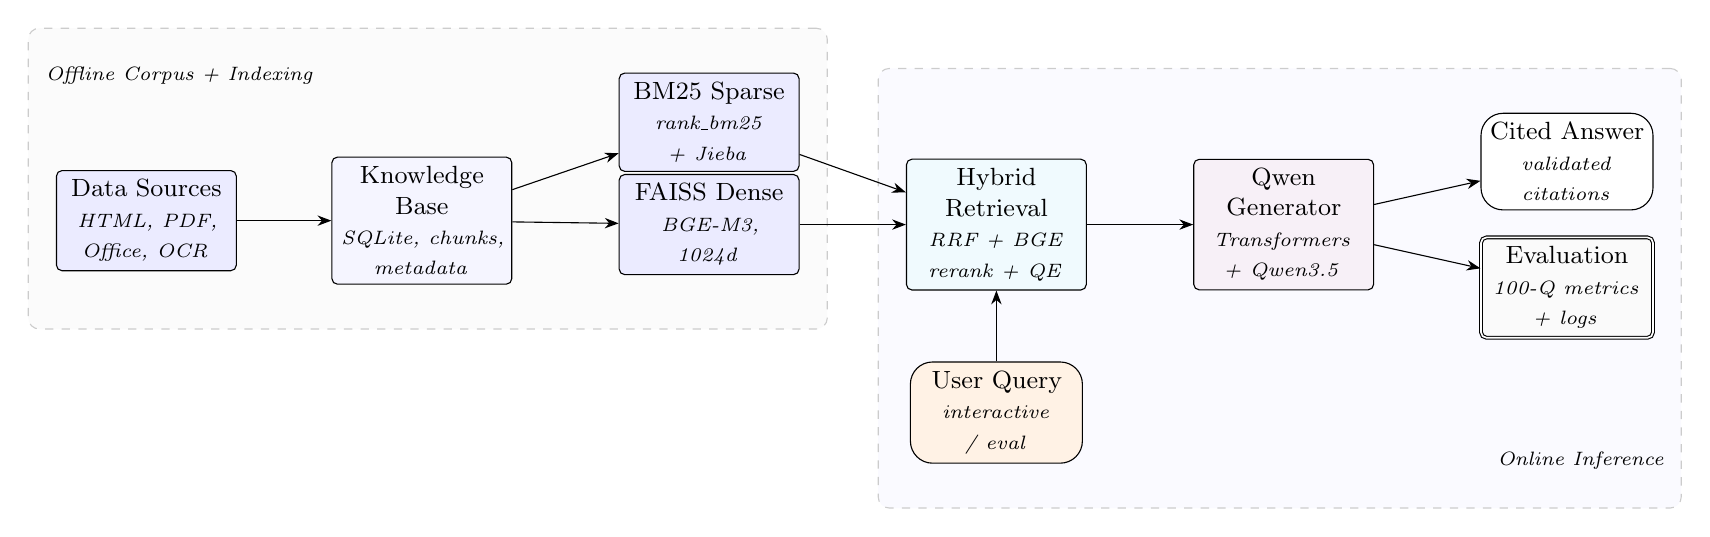
\begin{tikzpicture}[
  >={Stealth[length=5pt]},
  every node/.style={font=\small, align=center, minimum height=1.0cm, minimum width=1.95cm},
  box/.style={draw, rounded corners=2pt, fill=#1, text width=2.05cm},
  box/.default={blue!4},
  stadium/.style={draw, rounded corners=8pt, fill=#1, text width=1.95cm},
  stadium/.default={orange!8},
  dbox/.style={draw, double, rounded corners=2pt, fill=gray!4, text width=1.95cm},
]
% Column 1: Data Sources
\node[box=blue!8] (src) {Data Sources\\\scriptsize\textit{HTML, PDF, Office, OCR}};

% Column 2: Knowledge Base
\node[box, right=1.2cm of src] (kb) {Knowledge Base\\\scriptsize\textit{SQLite, chunks, metadata}};

% Column 3: Indexes
\node[box=blue!8, right=1.35cm of kb, yshift=1.25cm] (bm25) {BM25 Sparse\\\scriptsize\textit{rank\_bm25 + Jieba}};
\node[box=blue!8, right=1.35cm of kb, yshift=-0.05cm] (faiss) {FAISS Dense\\\scriptsize\textit{BGE-M3, 1024d}};

% Column 4: Hybrid Retrieval
\node[box=cyan!6, right=1.35cm of faiss] (ret) {Hybrid Retrieval\\\scriptsize\textit{RRF + BGE rerank + QE}};
\node[stadium=orange!10, below=0.9cm of ret] (query) {User Query\\\scriptsize\textit{interactive / eval}};

% Column 5: Generator
\node[box=violet!6, right=1.35cm of ret] (gen) {Qwen Generator\\\scriptsize\textit{Transformers + Qwen3.5}};

% Column 6: Outputs (stacked)
\node[stadium=white, draw, right=1.35cm of gen, yshift=0.8cm] (out) {Cited Answer\\\scriptsize\textit{validated citations}};
\node[dbox, right=1.35cm of gen, yshift=-0.8cm] (eval) {Evaluation\\\scriptsize\textit{100-Q metrics + logs}};

% Edges
\draw[->] (src) -- (kb);
\draw[->] (kb) -- (bm25);
\draw[->] (kb) -- (faiss);
\draw[->] (bm25) -- (ret);
\draw[->] (faiss) -- (ret);
\draw[->] (query) -- (ret);
\draw[->] (ret) -- (gen);
\draw[->] (gen) -- (out);
\draw[->] (gen) -- (eval);

% Background groupings
\begin{scope}[on background layer]
  \node[draw=gray!40, dashed, rounded corners=4pt, fill=gray!3,
        fit=(src)(kb)(bm25)(faiss), inner xsep=10pt, inner ysep=16pt] (offlinebox) {};
  \node[draw=gray!40, dashed, rounded corners=4pt, fill=blue!2,
        fit=(query)(ret)(gen)(out)(eval), inner xsep=10pt, inner ysep=16pt] (onlinebox) {};
  \node[font=\scriptsize\itshape, anchor=north west] at ([xshift=3pt,yshift=-3pt]offlinebox.north west)
        {Offline Corpus + Indexing};
  \node[font=\scriptsize\itshape, anchor=south east] at ([xshift=-3pt,yshift=3pt]onlinebox.south east)
        {Online Inference};
\end{scope}
\end{tikzpicture}%
}%
\caption{System architecture. Offline indexing builds sparse and dense indexes from official sources. Online inference retrieves, reranks, and generates a citation-constrained answer.}
\label{fig:architecture}
\end{figure}

\paragraph{Query-to-answer flow.}
At inference time, the user submits a question through the interactive interface or the batch evaluator. In dense mode, the system embeds the question with BGE-M3 and searches the dense vector index. In optimized hybrid mode, it retrieves sparse and dense candidates, optionally includes conservative expanded queries, fuses rankings with reciprocal rank fusion, applies bounded local reranking, and de-duplicates repeated source variants before selecting the final top contexts.

\paragraph{Context and answer flow.}
The selected contexts are converted into numbered source blocks containing the source title, address, trace reference, and text. The local Qwen generator receives only these blocks plus the user question; the prompt requires same-language answering, numbered citations, exact label-value preservation, and insufficient-evidence refusal when the sources do not support the answer. After generation, citation validation, repair prompting, and deterministic fallback decide whether to return a cited answer or an evidence-insufficient response. The interface displays the answer and source table, while evaluation runs write per-question traces, aggregate metrics, manual-review queues, and spreadsheet exports.

\section{Implementation Details}

This section details the two layers introduced above. We first describe the retrieval components that surface official evidence, then the generation components that turn that evidence into cited answers, and finally the shared interface and evaluation runtime through which both are exercised.

\subsection{Retrieval Components}

\paragraph{Index representation.}
The retrieval stack has two complementary indexes over the same official-source chunks. The sparse index uses BM25 with a tokenizer that combines ASCII/code-like tokens with Jieba Chinese segmentation, which makes exact identifiers such as course codes, room numbers, faculty names, and Chinese administrative terms directly searchable. The dense index uses BGE-M3 through SentenceTransformers. During indexing, each chunk is represented by an enriched retrieval field containing the page title, category, source address tokens, and chunk text; the vectors are normalized 1024-dimensional embeddings and are stored in a FAISS inner-product index. This enriched field is used only for matching. The answer context shown to the generator remains the original extracted official-source text, which avoids exposing synthetic metadata as answer evidence.

\paragraph{Dense and sparse query handling.}
For the before-optimization dense baseline, the runtime embeds the raw user question with the same BGE-M3 encoder and retrieves the five nearest chunks from FAISS. For the sparse channel, the query is tokenized with the same mixed English/Chinese tokenizer used at index time, and the BM25 candidate list is restricted to chunks that contain at least one query token. This simple filtering matters in a mixed corpus: it prevents high-scoring but query-disconnected BM25 artifacts from entering the hybrid candidate pool while preserving exact-match evidence for names, course identifiers, and page-specific phrases.

\paragraph{Hybrid retrieval strategy.}
The optimized retriever runs sparse and dense search in parallel, then fuses their ranked lists with reciprocal rank fusion. In the report-facing optimized condition, both channels retrieve a deeper candidate pool before fusion; the dense list receives 1.5$\times$ the sparse weight because dense retrieval was empirically stronger after index enrichment. The fused list is then diversified by normalized source address, document identity, SIST article identifier, and text hash, with at most one final context from the same source family. This de-duplication is important for generation because a top-five context window filled with near-duplicate chunks leaves no room for the second or third source needed by multi-field questions.

\paragraph{Reranking and query expansion.}
The final hybrid configuration applies a bounded local cross-encoder reranker rather than reranking the entire candidate list. It preserves the strongest fused candidates, reranks only the next small suffix with a local BGE reranker on GPU, and then selects the final five contexts. Conservative query expansion is applied only on the retrieval side: a local Qwen3-0.6B rewrite supplies one additional query per benchmark question, but the expanded text is filtered to stay close to the original question and is never inserted into the answer prompt or cited. This design keeps the benefit of lexical reformulation while avoiding the observed HyDE-style failure mode where generated pseudo-evidence introduced unsupported offices, emails, or institution names.

\subsection{Generation Components}

\paragraph{Local answer model.}
The generation path uses the same retriever interface for both dense and hybrid answer modes, then passes the selected evidence to a self-hosted Qwen-family causal language model loaded with Transformers. The dense generation baseline reported in this paper uses a local Qwen3.5-9B checkpoint, GPU inference, a five-context retrieval window, deterministic decoding, and a 1{,}024-token maximum answer budget. The model identifier is therefore a reproducibility descriptor, not a hosted API dependency; all answer runs use local files and offline execution.

\paragraph{Answer context selection.}
Before prompting the generator, the answerer reorders and trims retrieved contexts for answer synthesis. Contexts receive lightweight metadata scores from year overlap, exact date overlap, anchor-term overlap, program/course terms, contact evidence, and degree-plan cues; an optional local answer-side reranker can add cross-encoder scores. For long chunks, the system selects query-relevant local evidence windows and nearby sibling chunks from the same document or source. It also appends structured bindings for table-like evidence so that rows such as credit totals, offices, emails, and formula components remain attached to their labels. The citation numbers remain the original retrieval ranks even when the answer context order changes, so citations still map directly to the displayed source table.

\paragraph{Prompt template.}
The answer prompt is the following two-message chat template, with the question and numbered source blocks filled at runtime:
\begin{quote}
\small
\textbf{System message.}\\
You are a local RAG answer generator for official ShanghaiTech/SIST sources.\\
Answer in the same language as the user question.\\
Use only the provided sources. Do not use outside knowledge.\\
Preserve label-value bindings exactly; do not copy totals into adjacent rows or fields.\\
For formulas, preserve the source year's components and weights exactly.\\
Every factual paragraph must include at least one numbered citation like [1].\\
If the question asks for multiple fields or items, answer every requested field found in sources.\\
If the sources do not contain enough evidence, say that the evidence is insufficient.\\
Write only the final answer. Do not copy source metadata or prompt text.

\medskip
\noindent\textbf{User message.}\\
Question: \emph{\{user question\}}\\
Sources:\\
\emph{\{for each selected source\}}\\
{[}\emph{rank}{]} \emph{\{source title\}}\\
URL: \emph{\{source address\}}\\
chunk\_id: \emph{\{chunk identifier\}}\\
trace\_ref: \emph{\{retrieval trace reference\}}\\
TEXT:\\
\emph{\{official-source context text\}}
\end{quote}
For Qwen models that support chat templates, the runtime wraps these two messages with the tokenizer's chat template and disables thinking; otherwise it falls back to the same fields followed by an explicit ``Answer:'' marker.

\paragraph{Validation and recovery.}
The system treats fluent text as a draft rather than an automatically accepted answer. A generated answer is rejected if it leaks prompt fields, lacks valid citations, cites a non-retrieved source number, declares insufficient evidence without substantive facts, drops required contact/profile/credit fields, breaks label-value bindings, or reports unsupported formula values. After a rejection, one local repair pass sees the same numbered contexts and the rejected draft, and must return either a strict cited answer or an explicit insufficient-evidence status. If repair fails, deterministic source-derived recovery handles compact facts such as office/email pairs, addresses and postcodes, course teachers, dates, credit values, admissions fields, and short list answers. Only outputs that pass the same citation and leakage checks are returned as answered; otherwise the final status is evidence insufficient.

\subsection{Interface and Evaluation Runtime}

\paragraph{Interactive interface.}
The Gradio app exposes the same runtime path used by evaluation. It includes question input, retrieval-mode selection, a top-$k$ control, retrieval-only inspection, an answer panel, status messages, and source tables. If no local generator checkpoint is configured, the interface still runs as a retrieval-inspection tool, which is useful for auditing evidence quality independently from generation quality.

\paragraph{Batch evaluation.}
The evaluator consumes the structured 100-question benchmark and can run retrieval-only, answer-only, or paired retrieval-and-answer experiments. Each question records its category, language, expected answer, acceptable official sources, evidence snippets, grading notes, and judge type. Retrieval records store observed source addresses, top titles, packed contexts, fusion/reranking traces, and source metrics. Answer records additionally store the generated text, cited sources, answer status, generation path, rejection reason, fallback source rank when applicable, latency, and manual-review exports. The dense and optimized generation runs are compared under this shared protocol, with final correctness taken from the before/after generation CSV after manual labels are applied.

\section{Optimization}
\label{sec:optimization}

Optimization follows the two-layer structure of the system: we first improve evidence coverage at the retrieval layer, then improve answer faithfulness at the generation layer. We present each as a controlled study so that every change is tied to a specific failure mode rather than to a single end-to-end score.

\subsection{Retrieval-Layer Optimization}
\label{sec:retrieval-optimization}

The retrieval study isolates the contribution of each hybrid component by adding it on top of the previous accepted configuration, starting from a dense-only reference condition. That reference embeds the user query with BGE-M3, searches a dense vector index, and returns the top five chunks by semantic similarity, with no sparse matching, rank fusion, source de-duplication, enriched index text, reranking, or query expansion. It is a deliberately strong semantic baseline, which is precisely why its failures are informative: it misses exact course codes, faculty names, and source-address cues, and on multi-source questions its top-five window is easily consumed by near-duplicate chunks. Each subsequent row in the ablation targets one of these gaps.

We use the 100-question structured set, the same corpus snapshot, and a five-context retrieval budget throughout. URL and expected-source aliases are canonicalized for both conditions so that metrics reflect retrieval behavior rather than harmless source-address variants. The report-facing dense baseline is therefore rescored under the same canonicalization policy as the final hybrid system.

Table~\ref{tab:retrieval-fix-path} reports the controlled retrieval ablation path under this shared protocol.

\begin{table}[H]
\centering
\scriptsize
\setlength{\tabcolsep}{3.5pt}
\caption{Controlled retrieval ablation path. Rows show the main successful changes after the canonicalized dense baseline. Metrics are retrieval-only evidence metrics.}
\label{tab:retrieval-fix-path}
\begin{tabular}{lp{0.32\linewidth}rrrr}
\toprule
Condition & Main change relative to prior accepted condition & Hit@1 & Hit@5 & MRR@5 & Latency (s) \\
\midrule
Dense baseline & Dense-only FAISS retrieval with BGE-M3; no hybrid fusion or reranking & 0.52 & 0.74 & 0.594833 & 2.035649 \\
Hybrid fusion & Add BM25 and dense candidates with RRF under shared source canonicalization & 0.56 & 0.71 & 0.623167 & 2.882323 \\
Enriched indexing & Enrich index text with title, category, source address, path tokens, and chunk text & 0.64 & 0.80 & 0.705833 & 2.948884 \\
Weighted fusion & Give the dense rank list 1.5$\times$ the weight of the sparse rank list in RRF & 0.64 & 0.82 & 0.710833 & 2.989514 \\
Source diversity & Enforce strict final source diversity to avoid repeated source variants & 0.66 & 0.85 & 0.735333 & 2.969989 \\
Selective reranking (GPU) & Move the same selective reranker to GPU inference; ranking unchanged & 0.65 & 0.88 & 0.748333 & 5.141354 \\
Conservative query expansion & Add local Qwen query expansion before hybrid fusion & 0.67 & 0.89 & 0.757833 & 8.389798 \\
\bottomrule
\end{tabular}
\end{table}

\paragraph{From dense baseline to hybrid retrieval.}
The first optimization axis is adding a sparse channel. Dense retrieval captures semantic similarity, but the evaluation set contains many questions whose evidence depends on exact identifiers: course codes, faculty names, office rooms, admission program names, and URL-specific announcements. Hybrid retrieval adds BM25 candidates and fuses sparse and dense rankings with RRF. The first hybrid control already improves top-rank quality over dense under canonicalized evaluation, raising hit@1 from 0.52 to 0.56 and MRR@5 from 0.594833 to 0.623167. Its hit@5 is lower than dense at this stage, which shows that hybrid fusion alone is not sufficient; the later fixes are needed to recover broad top-five coverage.

\paragraph{Enriched index text.}
The largest single retrieval gain comes from changing the indexed representation rather than the displayed evidence. BM25 tokenization and dense embeddings are built from an enriched text field containing the title, category, canonical URL, URL slug/path tokens, and raw chunk text. Display snippets and packed contexts still use the original official-source text. This helps questions whose answer-bearing page can be identified by page title, category, or URL path even when the body chunk is short or table-like. Hybrid hit@5 rises from 0.71 to 0.80, and MRR@5 rises from 0.623167 to 0.705833.

\paragraph{Weighted rank fusion.}
After enrichment, dense retrieval remains more reliable than sparse retrieval for many semantic questions. The weighted-fusion variant keeps the same candidate pools and index text, but gives the dense rank list 1.5$\times$ the weight of the sparse rank list in RRF. This is a small but clean ranking adjustment: hybrid hit@5 improves from 0.80 to 0.82, MRR@5 improves from 0.705833 to 0.710833, and dense retrieval is unchanged because this change only affects hybrid fusion.

\paragraph{Strict source diversity.}
Several failures came from repeated source variants occupying multiple top-five slots. The source-diversity stage caps final output to one item per normalized source, document, and article family. This increases hybrid hit@5 to 0.85 by replacing repeated variants with additional distinct sources. The tradeoff is that nDCG@5 and precision@5 can drop slightly when repeated relevant chunks are replaced by diverse but non-relevant sources. This is still desirable for RAG context packing because a generator benefits from seeing distinct evidence sources.

\paragraph{Selective local reranking.}
A full top-50 cross-encoder reranker was tested but rejected as the default path: it raised hit@5 only to 0.86 while sharply hurting hit@1, MRR@5, nDCG@5, and CPU latency. The accepted reranking stage therefore preserves the fused top two candidates and reranks only a bounded top-20 suffix with a local BGE reranker. This keeps most first-rank quality while improving coverage: hit@5 rises from 0.85 to 0.88, source recall@5 rises to 0.853333, MRR@5 rises to 0.748333, and nDCG@5 rises to 0.738153. GPU inference is then used as a runtime optimization, preserving the exact ranking while reducing latency from 33.603731 seconds to 5.141354 seconds per query.

\paragraph{Conservative query expansion.}
The final accepted retrieval-ranking change adds one local Qwen3-0.6B rewrite per question. The rewrite is used only as an additional retrieval query; it is not inserted into the answer context and cannot be cited. A direct HyDE-style smoke test hallucinated unsupported offices, emails, and institution names, so the accepted version is deliberately conservative: generated terms are filtered back to the original question vocabulary. This improves hybrid hit@1 from 0.65 to 0.67, hit@5 from 0.88 to 0.89, MRR@5 from 0.748333 to 0.757833, and nDCG@5 from 0.738153 to 0.753315. The cost is latency: the final hybrid system averages 8.389798 seconds per query because the expanded query triggers an additional dense candidate pass.

\begin{table}[H]
\centering
\scriptsize
\setlength{\tabcolsep}{3.5pt}
\caption{Report-facing retrieval-only before/after comparison on the 100-question set. Metrics measure expected official-source evidence quality, not final generated-answer correctness.}
\label{tab:retrieval-main}
\begin{tabular}{lrrrrrr}
\toprule
Condition & Hit@1 & Hit@5 & Recall@5 & MRR@5 & nDCG@5 & Precision@5 \\
\midrule
Before: dense baseline, rescored & 0.52 & 0.74 & 0.723333 & 0.594833 & 0.614946 & 0.172 \\
After: optimized hybrid retriever & \textbf{0.67} & \textbf{0.89} & \textbf{0.858333} & \textbf{0.757833} & \textbf{0.753315} & \textbf{0.196} \\
Delta & +0.15 & +0.15 & +0.135000 & +0.163000 & +0.138369 & +0.024 \\
\bottomrule
\end{tabular}
\end{table}

Overall, the optimized retriever improves every report-facing retrieval metric over the dense baseline. Expected source hit@5 rises from 0.74 to 0.89, meaning that 15 additional questions surface at least one expected official source in the top five retrieved contexts. MRR@5 rises from 0.594833 to 0.757833, showing that expected sources are also ranked earlier, not merely added at the bottom of the context window. The final optimization stack is therefore not a single trick; it combines exact sparse recall, dense semantic recall, richer index text, rank-fusion calibration, source diversity, bounded local reranking, GPU runtime support, and conservative query expansion.

\subsection{Generation-Layer Optimization}
\label{sec:generation-optimization}

Generation optimization targets a different bottleneck from retrieval optimization: the generator must convert retrieved official evidence into complete, cited answers without adding unsupported facts. The dense Qwen3.5 baseline shows why this layer needs separate treatment. Among the 28 automatically incorrect dense-generation answers, final manual labels recover five loose-correct answers, but 15 remain partial and 15 both retrieved and cited an expected official source while still missing required facts. We therefore optimized the answer layer as a guarded evidence-synthesis module rather than treating the local language model output as the final answer by default.

\begin{table}[H]
\centering
\scriptsize
\setlength{\tabcolsep}{3pt}
\caption{Generation-layer optimization axes motivated by dense-baseline failure analysis. These changes improve answer grounding and completeness; aggregate before/after answer correctness is reported in Table~\ref{tab:generation-baseline}.}
\label{tab:generation-optimization-axes}
\begin{tabular}{@{}p{0.15\linewidth}p{0.23\linewidth}p{0.31\linewidth}p{0.20\linewidth}@{}}
\toprule
Axis & Failure addressed & Design & Expected effect \\
\midrule
Evidence-aware context selection & Correct source retrieved, but the needed row, sibling chunk, or label-value pair is weakly exposed & Reorder and trim retrieved contexts using year, date, program, contact, and table cues while preserving citation identities & Better support for curriculum tables, contact profiles, and multi-field pages \\
Prompt and decoding discipline & Fluent answers omit citations, mix unsupported knowledge, or copy source metadata & Use deterministic decoding, same-language answering, citation requirements, and explicit label-value and formula preservation instructions & More reproducible and citation-constrained drafts \\
Guarded answer acceptance & A plausible draft may still be uncited, incomplete, stale, or inconsistent with the cited evidence & Reject invalid citations, prompt leakage, unsupported insufficiency claims, missing required fields, and broken table bindings before accepting an answer & Fewer unsupported final answers and clearer abstentions \\
Model-first recovery and structured fallback & The model cites the right page but misses compact facts such as offices, credits, suppliers, dates, or list items & Try one constrained local repair pass, then synthesize short cited answers from source-derived evidence when the facts are explicit & Recovery for compact official facts without using answer keys \\
Diagnostic separation & Retrieval, citation, generation, and grading errors can be confused in aggregate accuracy & Track retrieved-source hit, cited-source hit, answer-synthesis misses, abstentions, and manual-review outcomes separately & Cleaner attribution of remaining failures \\
\bottomrule
\end{tabular}
\end{table}

\paragraph{Evidence-aware context selection.}
The first generation-side optimization is to change what the model sees after retrieval without changing the retrieved top-five evidence set. Retrieved contexts are reordered and locally expanded using question-relevant signals such as target year, exact date, program name, course terms, contact terms, and table-like labels. This addresses evidence-span misses in which the correct page is retrieved, but the answer-bearing row or neighboring chunk is not salient in the prompt. The design preserves the original citation numbers, so a generation-side ordering change does not obscure which retrieved source supports each answer sentence.

\paragraph{Guarded answer acceptance.}
The second optimization treats the local model output as a draft that must pass grounding checks before it becomes the final answer. The answer is rejected when it lacks valid numbered citations, cites unavailable sources, leaks prompt metadata, declares insufficiency despite available cited facts, drops requested fields, or breaks table label-value bindings. A constrained repair pass receives the same official contexts and must either produce a supported cited answer or abstain explicitly. This choice is intentionally conservative: for official-source question answering, an evidence-insufficient answer is preferable to a fluent answer grounded in the wrong year, program, or field.

\paragraph{Structured recovery for compact facts.}
The third optimization adds deterministic recovery for facts that are explicit in the cited sources but frequently missed by free-form generation. This recovery covers compact institutional facts such as office and email pairs, address and postcode fields, course teachers, dates, degree-plan credit values, supplier names, and short list answers. It is not an answer-key shortcut: it uses only the retrieved official contexts and must pass the same citation and leakage validation as model-written text. This design directly targets the dominant dense-baseline failure family, where the system cited the right page but omitted numeric table values or answered only one field of a multi-field question.

\paragraph{Evaluation implications.}
These optimizations also clarify how generation should be evaluated. Retrieved expected-source hit@5 measures whether official evidence was surfaced, cited expected-source hit measures whether the final answer used that evidence, and answer correctness measures whether the final text contains the required facts. Keeping these diagnostics separate prevents a retrieval improvement from being overstated as answer accuracy and prevents evaluator loosening from being mistaken for system improvement. The final comparison therefore reports correct answers after manual review, and it keeps source-retrieval and citation-grounding diagnostics separate from answer accuracy.

\section{Results}

\subsection{Retrieval Results}

Table~\ref{tab:retrieval-main} reports the primary retrieval comparison, and the message is uniform: the optimized hybrid retriever dominates the dense-only before-optimization condition on every metric --- top-rank quality, top-five coverage, recall, MRR, nDCG, and precision. The improvement is not a marginal reordering but a substantial gain in how often, and how early, official evidence reaches the context window.

A per-question breakdown confirms that this aggregate gain is not an averaging artifact. Table~\ref{tab:failure-taxonomy} partitions the benchmark by which condition surfaces an expected source, isolating the questions the optimization helps from the few it harms.

\begin{table}[H]
\centering
\small
\caption{Top-five expected-source overlap after the optimized hybrid retriever.}
\label{tab:failure-taxonomy}
\begin{tabular}{lrp{0.58\linewidth}}
\toprule
Result type & Count & Interpretation \\
\midrule
Both hit & 81 & Both retrieval conditions surface at least one expected official source. \\
Both miss & 7 & The current corpus or ranking signals are insufficient for the expected source. \\
Dense-only hit & 4 & Hybrid ranking or diversification displaces a useful dense result. \\
Hybrid-only hit & 8 & Optimization adds expected evidence that dense retrieval misses. \\
\bottomrule
\end{tabular}
\end{table}

The remaining failures are not dominated by missing corpus files. For checked disputed questions, expected URLs are often present in the enriched chunk index. The harder cases involve ranking, Chinese/English sibling pages, list pages versus detail pages, faculty profile variants, and course-table or faculty-course join questions that require stronger structured signals than chunk similarity alone.

\subsection{Generation Results}

The generation results answer a sharper question than the retrieval results: once the same evidence is available, does the guarded answer layer turn it into more correct answers? Table~\ref{tab:generation-baseline} reports the final before/after answer-generation comparison from the 100-question generation CSV, and its central tension is that final correctness rises even though one grounding diagnostic stays flat.

\begin{table}[H]
\centering
\small
\caption{Before/after Qwen3.5 generation results. Correct answers use the final reviewed labels in the comparison CSV. Optimized source/citation diagnostics are averaged over the 99 rows with populated after-run diagnostic fields.}
\label{tab:generation-baseline}
\begin{tabular}{lrr}
\toprule
Metric & Dense generation baseline & Optimized generation \\
\midrule
Correct answers & 59/100 & 69/100 \\
Evidence-insufficient answers & 18/100 & 14/100 \\
Remaining wrong or incomplete answers & 23/100 & 17/100 \\
Retrieved expected source hit@5 & 0.740 & 0.808 \\
Cited expected source hit@5 & 0.670 & 0.677 \\
Answer-synthesis miss rate & 0.050 & 0.091 \\
Average latency & 16.095 s & 24.200 s \\
\bottomrule
\end{tabular}
\end{table}

The optimized generation system improves final answer correctness but does not remove all answer-side bottlenecks. Correct answers rise from 59/100 to 69/100. The optimized run also reduces evidence-insufficient answers from 18 to 14 and reduces remaining wrong or incomplete answers from 23 to 17. At the same time, cited expected-source hit@5 is nearly flat and answer-synthesis miss rate increases from 0.050 to 0.091, showing that the gains come from better answer construction in selected cases rather than a uniform improvement in every grounding diagnostic. The latency cost is also visible: average answer latency rises from 16.095 seconds to 24.200 seconds.

Table~\ref{tab:generation-cases} selects representative cases from the final comparison CSV. The examples were chosen to cover distinct optimization effects rather than to duplicate the aggregate score.

\begingroup
\scriptsize
\setlength{\LTpre}{4pt}
\setlength{\LTpost}{4pt}
\setlength{\tabcolsep}{3pt}
\newcommand{\casecell}[1]{\begin{minipage}[t]{\linewidth}\raggedright\sloppy #1\end{minipage}}
\begin{longtable}{p{0.05\linewidth}p{0.26\linewidth}p{0.29\linewidth}p{0.29\linewidth}}
\caption{Representative case studies from the final before/after generation artifacts. Questions and answers are copied from the dense and optimized Qwen3.5 runs.}
\label{tab:generation-cases}\\
\toprule
Case & Question & Dense generation answer & Optimized generation answer \\
\midrule
\endfirsthead
\toprule
Case & Question & Dense generation answer & Optimized generation answer \\
\midrule
\endhead
\bottomrule
\endfoot
q010 &
\casecell{我是一名对电动汽车和光伏储能方向非常感兴趣的学生，希望在信息学院找一位入选过“上海领军人才”的教授做我的导师，请问我最应该联系哪位老师？} &
\casecell{证据不足：当前检索到的官方来源不足以回答这个问题。} &
\casecell{您最应该联系**王浩宇**教授。\par
根据提供的资料，王浩宇教授完全符合您的所有要求：\par
1. **入选“上海领军人才”**：资料明确指出他是“上海领军人才”[1][2]。\par
2. **研究方向高度匹配**：他的研究方向包括“电动汽车”和“光伏”（资料中提及“算力电源、电动汽车”[1][2]，且团队有专门针对“车顶光伏充电系统”的研究成果 [3]）。\par
3. **具体研究成果**：他团队提出了适用于**800V电动汽车车顶光伏充电**的新方案，解决了高升压比、低输入纹波等关键技术问题，并发表了相关论文 [3]。此外，他还拥有多项关于电池均衡、光伏供能及电动汽车变换器的专利 [1][2]。\par
4. **导师资格**：他是信息学院的长聘正教授、博导 [1][2]。\par
建议您在联系前，可参考信息学院研招办的联系方式（邮箱：admission.\allowbreak sist@\allowbreak shanghaitech.\allowbreak edu.\allowbreak cn）[4]，或直接通过其个人主页（https://sist.\allowbreak shanghaitech.\allowbreak edu.cn/\allowbreak wanghy/\allowbreak main.htm）[2] 获取更详细的联系方式。} \\
\midrule
q032 &
\casecell{寇煦丰教授（Xufeng Kou）和周平强教授（Pingqiang Zhou）在信息科学与技术学院均担任副院长（Associate Dean）职务。请问他们两位老师在信息学院大楼（SIST Building）的官方办公室房间号分别是多少？} &
\casecell{根据提供的官方信息，两位老师在信息科学与技术学院（SIST）大楼的办公室房间号如下：\par
* **周平强教授（Pingqiang Zhou）**：担任副院长（vice dean），其办公室位于 **Room 1A-219** [1][2][5]。\par
* **寇煦丰教授（Xufeng Kou）**：担任副院长（assistant dean），其办公室位于 **Room 3-318** [3][4]。} &
\casecell{根据提供的官方来源，寇煦丰教授（Xufeng Kou）和周平强教授（Pingqiang Zhou）在信息科学与技术学院（SIST）的官方办公室房间号如下：\par
* **寇煦丰教授（Xufeng Kou）**：办公室位于 **Room 3-318, SIST Building** [2][3][5]。\par
*注：虽然来源 [5] 中曾出现 "Room 3-316" 和 "Room 3-318" 的文本片段，但明确标注其职务为 "Professor, Associate Dean" 且与 "Xufeng Kou" 直接关联的条目为 "Room 3-318, SIST Building" [5]。来源 [2] 和 [3] 也一致确认其办公室为 Room 3-318。*\par
* **周平强教授（Pingqiang Zhou）**：办公室位于 **Room 1A-221, SIST Building** [5]。\par
*注：来源 [1] 和 [4] 显示其邮箱和电话关联的地址为 "Room 1A-219"，但来源 [5]（PMICC 教师列表）明确将 "Professor, Associate Dean" 的 "Pingqiang Zhou" 与 "Room 1A-221" 对应。鉴于 [5] 是专门列出教师职务与房间号的列表，该信息更为直接对应其副院长职务的办公地点。*\par
**总结：**\par
* **Xufeng Kou**: Room 3-318\par
* **Pingqiang Zhou**: Room 1A-221} \\
\midrule
q039 &
\casecell{在2023年期间，信息学院机电能源平台针对共享仪器设备面向在校师生发布技能培训通知。其中，在当年的 10 月 28 日和 11 月 04 日这两个特定日期举办的培训，其核心针对的共享仪器分别叫什么名字？} &
\casecell{研究生招生介绍一览; Newsletter; 信息学院机电能源平台共享仪器技能培训; 发布时间：2023-03-15 [1].} &
\casecell{根据提供的来源，在2023年期间，信息学院机电能源平台发布的技能培训通知中，针对特定日期的共享仪器如下：\par
1. **10 月 28 日**：该日期的培训针对的共享仪器名为**可变温磁光克尔成像系统** [2]。\par
2. **11 月 04 日**：该日期的培训针对的共享仪器名为**低温磁光克尔成像** [2]。\par
*注：虽然来源 [1] 详细列出了2023年3月至4月的培训日程，但来源 [2] 的“技能培训”列表明确记录了2022年10月27日发布的关于10月28日“可变温磁光克尔成像系统”的培训通知，以及2023年2月6日发布的关于11月04日“低温磁光克尔成像”的培训通知。*} \\
\midrule
q065 &
\casecell{精密传感与智能检测实验室的研究方向、招生名额、联系邮箱和课题组组长分别是什么？} &
\casecell{email: 申请请联系yechf@shanghaitech.edu.cn [1].} &
\casecell{研究方向是无损检测、电磁测量与成像、电磁场与电路系统建模；招生名额是2-3个硕士或博士名额；联系邮箱是申请请联系yechf@shanghaitech.edu.cn；组长是叶朝锋。 [1]} \\
\midrule
q069 &
\casecell{2025级CS专业本科生在专业限选课程中，如果同时多修读了“电路基础加实验”和“信号与系统加实验”这组二选一课程，多出的学分会如何计入？同一规则还适用于哪一组二选一课程？} &
\casecell{根据提供的2020级计算机专业（CS）培养方案 [5]，在专业限选课程板块中，“电路基础加实验”（EE111+EE111L）和“信号与系统加实验”（EE150+EE150L）属于“至少二选一”的课程组。如果学生同时多修读了这两门课程，**多出的学分会记在本学科选修的31学分中**。\par
同一规则同样适用于该板块中的另一组二选一课程：**“操作系统”（CS130）和“人工智能”（CS181）**。如果多选这两门课，多余学分也将记在本学科选修的31学分中 [5]。\par
*注：2022级及2023级EE专业培养方案 [1][2][3] 中，对应课程组（电路基础、信号与系统）的规则为“至少三选二”，多余学分记在本学科选修的21学分中，但问题明确询问的是CS专业且涉及的具体课程组合（如“电路基础加实验”）主要出现在2020级CS方案中。*} &
\casecell{根据 2025 级 CS 专业培养方案 [4]，在专业限选课程板块中，“电路基础加实验”（EE111+EE111L）和“信号与系统加实验”（EE150+EE150L）为二选一课程。如果学生同时多修读了这两门课程，多出的学分会记在**本学科选修**（34 学分）中。\par
同一规则同样适用于**CS130**（操作系统 I）和**CS181**（人工智能 I）这组二选一课程，若多选，多余学分也将记在本学科选修的 34 学分中 [4]。} \\
\midrule
q090 &
\casecell{根据信息学院博士研究生招生列表页，在2026年4月22日、4月15日和3月17日分别列出的三条2026年博士招生相关公告标题是什么？} &
\casecell{证据不足：当前检索到的官方来源不足以回答这个问题。} &
\casecell{根据信息学院博士研究生招生列表页（来源 [3]），在指定日期列出的三条2026年博士招生相关公告标题如下：\par
* **2026年4月22日**：上海创芯学院\&上海科技大学2026年电子信息工程博士招生简介 [3]\par
* **2026年4月15日**：上海科技大学-北京通用人工智能研究院2026年联合培养博士生专项计划（“通计划”）-第二轮报名 [3]\par
* **2026年3月17日**：上海科技大学信息科学与技术学院2026年全日制工程类专业学位博士报名通知（第二轮） [3]} \\
\end{longtable}
\endgroup

The pattern in Table~\ref{tab:generation-cases} explains why the final generation result improves even though aggregate citation hit@5 does not improve. Some cases are genuine retrieval gains, such as routing a curriculum question to the correct year or recovering a dated admissions list. Other cases are answer-layer gains: the expected source was already retrieved and cited, but the baseline answer omitted required fields or failed to assemble compact facts from the cited context. The remaining errors show that this optimization is not complete; curriculum tables and long PDF-like evidence still produce wrong or insufficient answers in several questions.

\section{Discussion and Conclusion}

Our central finding is that official-source university QA improves only when retrieval and generation are optimized as two distinct layers and measured as two distinct layers. Treating the system as a single black box would have hidden where the gains and the remaining failures actually live; separating the layers is what makes both the progress and its limits legible.

At the retrieval layer, a carefully assembled local stack closes most of the evidence gap without any hosted API. Exact sparse matching, dense semantic matching, rank fusion, source diversity, selective reranking, and conservative query expansion are individually small, but together they raise expected source hit@5 from 0.74 to 0.89 on the structured 100-question benchmark and rank expected sources earlier rather than merely deeper. The lesson is that no single trick carries this task; robustness comes from covering complementary failure modes, since exact-identifier questions and semantic questions fail for different reasons.

At the generation layer, the downstream gain is smaller but confirms that better evidence is necessary, not sufficient. Correct answers rise from 59/100 to 69/100, evidence-insufficient answers fall from 18 to 14, and remaining wrong or incomplete answers fall from 23 to 17. These gains do not come from a stronger model but from disciplining a fixed one: answer-context selection surfaces the right row, completeness and citation checks reject ungrounded drafts, and source-derived recovery assembles compact facts that free-form generation drops. The same evidence, used more carefully, produces ten more correct answers.

These two stories are only separable because the evaluation refuses to conflate them. A retrieved source can be relevant while the generator still omits a required fact, cites the wrong block, or abstains; conversely, a fluent answer can read well while never citing the expected official source. By keeping retrieved evidence, cited evidence, answer text, final review labels, and assignment spreadsheet fields as distinct quantities, we ensure that a retrieval improvement is never overstated as answer accuracy and that evaluator loosening is never mistaken for system progress. We regard this discipline as transferable beyond this corpus: any official-source QA system that reports a single blended score risks attributing gains to the wrong layer.

\paragraph{Limitations.}
Our results are bounded in four ways. First, accuracy is bought with latency: the optimized generator is more correct but slower, with average answer latency rising from 16.095 seconds to 24.200 seconds, mostly from the additional expansion pass and reranking. Second, one optimized-run record lacks populated source and citation diagnostics, so after-run grounding rates are reported over the populated diagnostic rows rather than asserting a complete diagnostic field for every question. Third, time-sensitive questions are judged against a fixed corpus snapshot and the dates on the source pages, so a stale official page degrades both retrieval and answer quality regardless of system design. Fourth, and most informative for future work, the residual generation failures concentrate where cited official sources alone are insufficient: degree-plan tables, long PDF-like evidence, multi-field answer slots, and year- or program-specific constraints that must survive answer synthesis intact.

\paragraph{Future work.}
The limitations point directly at the next layer of work. On the answer side, the dominant remaining failure family motivates table-aware evidence expansion for degree plans, stronger multi-field completeness validation, year- and program-specific source routing, and citation-coverage repair that guarantees every required slot is grounded. On the retrieval side, the latency cost motivates caching the dense encoder across expanded queries and restricting expansion retrieval to sparse candidates when latency is constrained, while accuracy motivates contextual chunk enrichment with breadcrumbs and entity aliases and a dedicated audit of Chinese/English sibling pages and faculty/list page variants, kept separate from genuine retrieval changes so that ranking gains are not confused with corpus cleanup.

In conclusion, the implemented system meets the core requirements for an official-source, local-model RAG pipeline with an interactive interface and reproducible evaluation artifacts, and it does so through a two-layer design measured by a layered protocol. The evidence supports a strong retrieval-optimization result and a downstream generation result that improves correct answers by ten points over the dense generation baseline. More broadly, it argues that for high-stakes institutional QA, the discipline of separating evidence quality from answer correctness is as important as any single retrieval or generation technique.

\begin{thebibliography}{9}

\bibitem{lewis2020rag}
Patrick Lewis, Ethan Perez, Aleksandra Piktus, Fabio Petroni, Vladimir Karpukhin, Naman Goyal, Heinrich Kuttler, Mike Lewis, Wen-tau Yih, Tim Rocktaschel, Sebastian Riedel, and Douwe Kiela.
\newblock Retrieval-augmented generation for knowledge-intensive NLP tasks.
\newblock In \emph{NeurIPS}, 2020.

\bibitem{gao2023rag}
Yunfan Gao, Yun Xiong, Xinyu Gao, Kangxiang Jia, Jinliu Pan, Yuxi Bi, Yi Dai, Jiawei Sun, and Haofen Wang.
\newblock Retrieval-augmented generation for large language models: A survey.
\newblock \emph{arXiv preprint arXiv:2312.10997}, 2023.

\bibitem{johnson2019faiss}
Jeff Johnson, Matthijs Douze, and Herve Jegou.
\newblock Billion-scale similarity search with GPUs.
\newblock \emph{IEEE Transactions on Big Data}, 2019.

\bibitem{reimers2019sentencebert}
Nils Reimers and Iryna Gurevych.
\newblock Sentence-BERT: Sentence embeddings using Siamese BERT-networks.
\newblock In \emph{EMNLP-IJCNLP}, 2019.

\bibitem{robertson2009probabilistic}
Stephen Robertson and Hugo Zaragoza.
\newblock The probabilistic relevance framework: BM25 and beyond.
\newblock \emph{Foundations and Trends in Information Retrieval}, 2009.

\bibitem{cormack2009rrf}
Gordon V. Cormack, Charles L. A. Clarke, and Stefan Buettcher.
\newblock Reciprocal rank fusion outperforms Condorcet and individual rank learning methods.
\newblock In \emph{SIGIR}, 2009.

\bibitem{qwen2025}
Qwen Team.
\newblock Qwen3 technical documentation and model releases.
\newblock \url{https://qwenlm.github.io/}.

\bibitem{gradio}
Gradio Team.
\newblock Gradio documentation.
\newblock \url{https://www.gradio.app/docs}.

\end{thebibliography}

\end{CJK*}
\end{document}
